\section{Signal acceptance from asymmetric jet \Pt thresholds}

For a typical compressed model, Fig.~\ref{fig:asymMotivation} shows
the second jet \PT distribution for two different \HT bins. In the low
\HT case a large portion of the events are killed by requiring the
second jet to have $\ET>100\gev$.

We therefore add an new analysis category where the leading jet is
required to fulfil momenta of jet $\ET>100\gev$ and sub-leading jet
$40\gev<\ET<100\gev$. This new category results in new asymmetric jet
bins split also in $\njet$, $\nb$ and \HT. The asymmetric jet bin
results in much larger acceptance for monojet-type and ISR induced
event topologies like DM signals and compresses SUSY scenarios.  For
the simplified model T2tt with $m_{\rm stop}=425\gev$ and $m_{\rm
  LSP}=325\gev$, including these bins increases signal acceptance by
around a factor 3, for the DM models a factor of five is observed.
The addition of the asymmetric bin can only lead in combination to
improvements or constant sensitivities.

\begin{figure}[h!]
  \centering
  \subfigure[Second jet \PT for $200\gev<\HT<250\gev$, $\alphat>0.65$]{
    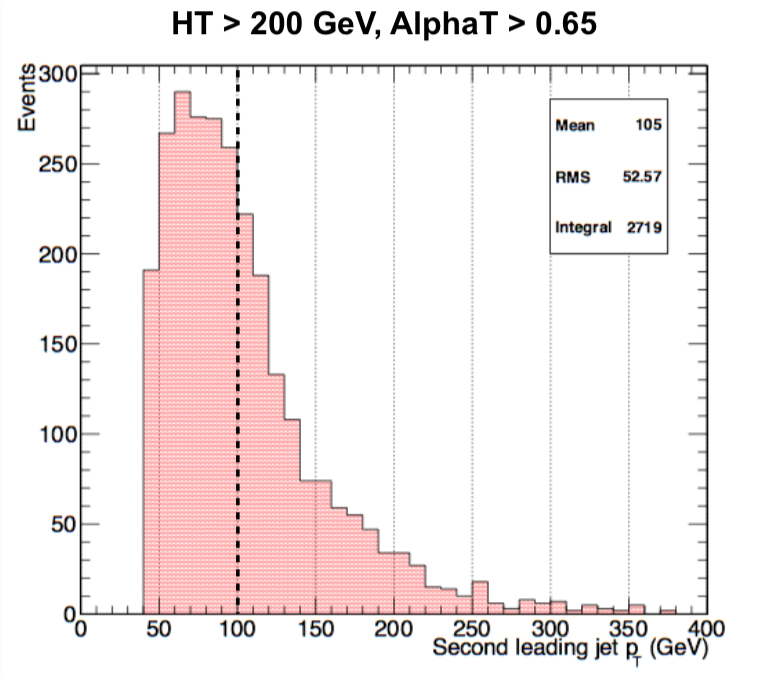
\includegraphics[width=0.5\textwidth]{figures/asymPlots/secondJetPtlowHT}
  }~~
  \subfigure[Second jet \PT for $400\gev<\HT>500\gev$, $\alphat>0.52$]{
    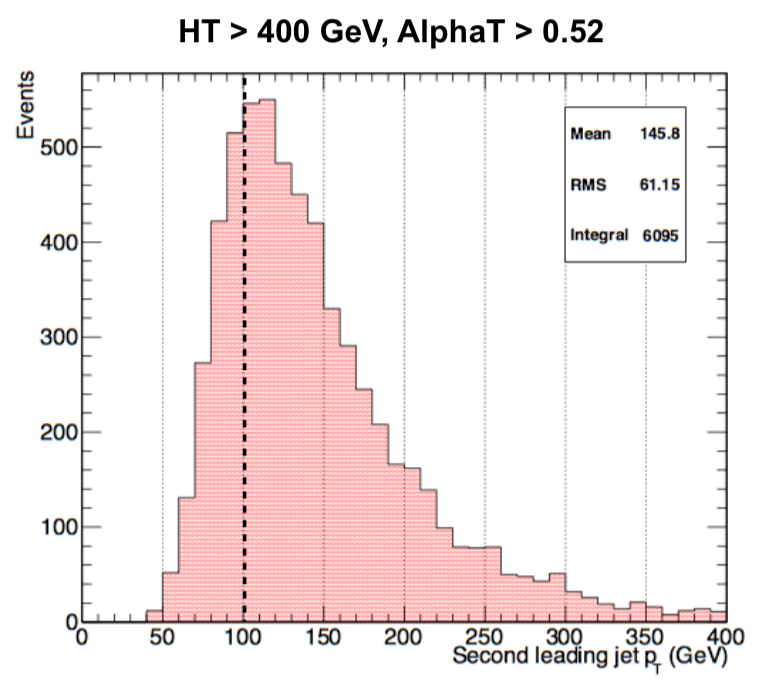
\includegraphics[width=0.5\textwidth]{figures/asymPlots/secondJetPthigherHT}
  }
  \\
  \caption{\label{fig:asymMotivation} The second leading jet \PT for
    different cases of \HT after a baseline signal selection:
    $\njet\geq2$, lead jet $\ET>100\gev$, lepton vetoes. Made with the
    T2tt ($m_{\rm stop}=425\gev$, $m_{\rm LSP}=325\gev$) simplified
    model sample.}
\end{figure}
